\documentclass[conference]{IEEEtran}

\usepackage[utf8]{inputenc}

\usepackage{multirow}
\usepackage[table,xcdraw]{xcolor}
\definecolor{Gray}{gray}{0.9}
\usepackage[pdftex]{graphicx}
\usepackage{pgfplots}
\DeclareUnicodeCharacter{2212}{−}
\usepgfplotslibrary{groupplots,dateplot}
\usetikzlibrary{patterns,shapes.arrows}
\pgfplotsset{compat=newest}

\usepackage[caption=false,font=footnotesize]{subfig}
\usepackage{numprint}
\usepackage{abbrevs}
\usepackage{algorithm}
\usepackage{algorithmic}
\usepackage{stfloats}
\usepackage{lipsum}
\usepackage{url}
\usepackage{parskip}
\usepackage[activate={true,nocompatibility},final,tracking=true,kerning=true,spacing=true,factor=1100,stretch=10,shrink=10]{microtype}
\usepackage{standalone}
\usepackage{tikz,pgf}
\usetikzlibrary{fit, bayesnet, arrows.meta, positioning, trees, decorations.pathreplacing,calligraphy, backgrounds}
\usepackage{array}
\usepackage{amsmath}
\usepackage{bm}
\usepackage{units}
\usepackage{cite}
\usepackage{makecell}
\usepackage{multirow}
\usepackage{colortbl}
\usepackage{booktabs}
\usepackage{tabu}
\usepackage{arydshln}
\usepackage{color}

\usepackage{pifont}
\newcommand{\cmark}{\ding{51}}%
\newcommand{\xmark}{\ding{55}}%

\begin{document}

\title{Prediction of Recurrent Flow Characteristics \\ Using Time Scale Ensemble Learning}

\author{\IEEEauthorblockN{Mike Petersen}
\IEEEauthorblockA{
Student-ID: 1221772\\
Fulda University of Applied Sciences\\
Email: mike.petersen@informatik.hs-fulda.de}
\and
\IEEEauthorblockN{Oliver Kovarna}
\IEEEauthorblockA{
Student-ID: 539151\\
Fulda University of Applied Sciences\\
Email: oliver.kovarna@informatik.hs-fulda.de}
}

\maketitle

\begin{abstract}
The exponential growth of Internet traffic requires increasingly efficient resource utilization within network systems by providing both integrative and fine-grained management of network components. Recent advancements combine software-defined networking concepts and machine learning approaches in order to analyze network traffic behavior and enable automatic derivation of network and service management decisions, such as dynamic path determination based on predictions of network characteristics. A key challenge in classifying network flows is the adaptation to unforeseen changes in the underlying distribution of the data stream. This phenomenon, known as concept drift, leads to the degradation of deployed models resulting in poor predictions and decision outcomes. In this context, we present a network traffic classification method based on online ensemble learning. Specifically, a flow data stream is partitioned based on a set of windows with different time scales. Within the life cycle of each time window, both inference and training of a DNN is performed in an online fashion. The scores from the respective time windows are consolidated using an ensemble strategy. In this way, temporal dependencies between data instances are addressed and concept drifts of different types and speeds should be handled. Experiments on real network data demonstrate the accuracy performance of our approach in comparison to a single online model.
\end{abstract}

\begin{IEEEkeywords} Traffic Engineering, Flow Prediction, Machine Learning, Ensemble Learning, Concept Drift \end{IEEEkeywords}

\IEEEpeerreviewmaketitle


\section{Introduction}\label{sec:introduction}
\subsection{Problem Statement}\label{sec:problem_statement}
In the context of \textit{network flow prediction}, machine learning approaches have recently emerged that enable accurate classification of network flow data and thus better management of network components and the incoming traffic. In many areas of the internet, providers of various services are challenged with a large volume of streaming data due to increasing link speeds and number of users. Since many unforeseen changes can occur in network traffic, it is necessary to process the data in an online fashion in order to detect drifts quickly and deal with them accordingly \cite{gama_concept_drift}. In general, unforeseen changes in data patterns are known as \textit{concept drift} \cite{gama_concept_drift}. Considering the different types of concept drift is important for further investigation. A sudden drift occurs after a short period of time and causes a direct change in the data distribution. With a gradual drift, the new concept replaces the old concept linearly. An incremental drift occurs step by step over a certain period of time. When an online model encounters one of these three types it should adapt to these concepts and try to restore the previous accuracy. In case of \textit{recurrent concepts}, a new concept is established only temporarily before restoring the old concept again. The different types of concept drift can happen at a certain point in time or can appear over a certain amount of time. Moreover, the concepts of these different types can transition into each other \cite{lu_concept_drift}. Deep Neural Networks (DNNs) usually are well qualified for the application within high volume data streams with drifts, because their architecture inherently allows an online classification. However, their online learning capability comes at cost as they suffer from a phenomenon called catastrophic forgetting (CF). The problem of CF refers to the complete elimination of previously learned information by a neural network, when exposed to new information \cite{MCC_1989, RAT_1990}. If the changes in the data statistics are recurrent drifts of high dynamic and intensity the model's performance can be degraded dramatically. The naive approach to cope with this challenge is to retain data in order to feed the network with old patterns that may get lost as the drift occurs. We assume that one way to address this problem is to support an online model with multiple offline models, each of which is based on an state from past time windows \cite{hardegen_predicting_2020}. The fact that ensemble learners are used for dealing with class imbalance or concept drift \cite{sage_ensemble_learning} supports the decision to organize such different models in form of an ensemble. In this way, the above-mentioned short-term unforeseen changes within the network traffic shall be adequately addressed by implementing a robust continuous adaptation for the model.

\subsection{Contributions}\label{sec:contributions}
\begin{itemize}
    \item We provide an overview of existing classification techniques that leverage the concept of multiple windows and highlight the differences with our approach.
    \item We perform online multi-class training and inference of a flow's bit rate by using an ensemble of DNNs in a streaming setup, where the state of each level $0$ model is based on a different sized time window.
    \item We compare the accuracy performance between a single online classifier and the ensemble on real network data.
    \item We provide the code for the implementation of the presented architecture.
\end{itemize}


\section{Related Work}\label{sec:related_work}
\subsection{Traffic Classification with Machine Learning}\label{sec:traffic_classification_with_machine_learning}

A comprehensive survey on the application of different machine learning paradigms and techniques to fundamental problems in networking is provided in \cite{boutaba2018comprehensive}. An overview that focuses on the subject of network traffic control, specifically discussing deep learning based routing in contrast to conventional routing, is given in \cite{fadlullah2017state}.

Poupart et al. \cite{poupart_online_2016} explore the application of different machine learning algorithms for network traffic prediction. By categorizing network traffic flows based on their predicted size into elephant and mice flows, the completion time of elephant flows is intended to be minimized. Seven features (source IP, destination IP, source port, destination port, protocol, server vs. client and size of the first three packets) are considered as input for the selected algorithms, which include an Online Bayesian Moment Matching (oBMM), a Gaussian Process Regression (GPR) and a Neural Network (NN). According to the classification results, mice flows are routed by equal cost multipath (ECMP) routing, while elephant flows are routed by least congested (LCR) routing. Consequently, the algorithms improve routing and scheduling, since flow sizes are already known at the beginning of a flow's life cycle. However, the runtime complexity of GPR and oBMM do not enable a scaled application in real network environments.

In \cite{malik_intelligent_2020}, Malik et al. have developed a SDN-based flow routing framework, acting as the application layer for network traffic classification via a northbound API. Processes within this architecture are divided into two phases. During the learning phase, network traffic flows are collected periodically and stored in a historical data store. A flow pattern analysis and feature extraction constructs a refined database, that is utilized for the training and evaluation of a deep learning classifier. The subsequent action phase attains and utilizes learned information for load balancing and routing. Finally, the SDN controller uses the learned knowledge for routing updates, optimising the network's performance and classifying the network traffic. The proposed framework is tested on the Moore dataset by classifying the network traffic into distinct application classes, showing effective and scalable classification results.

Hardegen et al. \cite{hardegen_flow-based_2019} propose a processing pipeline for a network-flow based throughput classification using deep neural networks (DNNs). Flows are categorized into three classes based on their predicted bitrate. For this purpose, the feature set containing the standard 5-tuple is additionally enriched with metadata (e.g. private/public prefixes, VLANs, ASNs) extracted from the internal and global topology. Besides the presentation of the classification pipeline, an in-depth analysis of the characteristics of the real-world network traffic data collected for the experiments is performed. The evaluations show that a multi-class bit rate prediction for streamed flow data is feasible with DNNs and that enriching the flows can contribute to a significant improvement in accuracy. 



\subsection{Multiple Window Approaches}
Li et al. \cite{li_multi-window_2017} introduce a windowing approach that is intended to improve the classification of imbalanced streaming data. The different windows represent the current batch of instances, the latest minority instances, and the ensemble classifier. By keeping a window of minority instances, the algorithm copes with imbalanced data streams. For the current batches, a sliding window approach is applied. The optimal window size is determined heuristically. Before classification, the weights of each sub-classifier are adjusted by calculating similarities of the current and last window used to train each sub-classifier. The classification is performed by a weighed majority voting strategy. Training of a new sub-classifier is performed as soon as the current ensemble classifier is imprecise concerning minority and majority classes.

The network intrusion detection system Kitsune \cite{mirsky_kitsune_2018} performs an anomaly detection by using multiple autoencoders on a bagged feature space. The utilization of damped windows that incrementally update the systems's statistics saves memory and runtime. This way, only the most recent occurrence within the packet channel is recorded. The framework includes a packet capturer, a packet parser, a feature extractor, a feature mapper and the anomaly detector KitNET. The feature vector is split into groups of attributes, which are each mapped to an autoencoder within the ensemble. The root mean squared error (RMSE) between the original instance and the reconstruction that is calculated by each autoencoder is used as input for a subsequent autoencoder that calculates the final anomaly score.

Lazarescu et al. \cite{lazarescu_2004_using} present an incremental learning algorithm in that predicts and adapts to real and   drifts using three different windows. While the smallest window deals with fast changing concepts, the largest window considers the slowest changing concepts. The input is labelled with a concept size and assigned to one of the windows. The small window's concept changes are used to determine the size changes of the other windows. The algorithm allows multiple hypotheses on the basis of recognised concepts and handles virtual drifts well. However, each concept requires an extra window, resulting in a high computational complexity. 

\subsection{Key Distinguishing Features}

\begin{itemize}
    \item We perform a supervised complete flow traffic classification in a true online fashion instead of splitting the input flows into subsets of train and test flows.
    \item The evaluation is conducted on a real world network traffic dataset that contains realistic network characteristics instead of using a synthetic dataset.
    \item Each window within the proposed architecture is provided with the full feature set but differ in the context of their timely state.
    \item Instead of explicitly detecting drifts in the data stream, the approach shall handle recurrent concepts by learning dependencies between the different windows by combining their results in a meta learner. 
\end{itemize}


\begin{figure*}[t]
\centering
\includestandalone[width=1\linewidth]{tikz/data_flow_diagram}
\caption{The high level system architecture of the flow processing pipeline depicting the data flow between the main components.}
\label{fig:system_architecture}
\end{figure*}

\newpage

\section{Flow Data Processing Pipeline}\label{sec:flow_data_processing_pipeline}
First, the high-level system architecture describing the data flow between the individual components is outlined (see Figure \ref{fig:system_architecture}). This is followed by a specification of the introduced components and their corresponding tasks. Thereby, the main system components from \cite{hardegen_flow-based_2019}, on which our implementation is largely based, are covered. Finally, the ensemble extensions are described. The implementation of this architecture is publicly available in a Git repository\footnote{\url{https://github.com/mikepetersyn/Flow-Data-Streaming-Client-Ensemble}}.


\subsection{Data Flow} \label{sec:data_flow}
Exported flows are collected by the \textit{NetFlow Collector} until a defined block size (default \numprint{100000}) is attained. The \textit{Flow Processor} then splits the block of flow records into disjoint subsets of equal size depending on the number of parallel processes being available. Each subset is passed to one of $n$ parallel \textit{Flow Processors}, which execute \textit{Aggregation}, \textit{Enrichment}, and \textit{Anonymization} functions. The subsets are then merged back into a block and compressed by the \textit{Flow Processor} and either passed to the \textit{Connection Handler} for further processing or exported as an offline dataset. The exported data can be replayed by a \textit{File Streamer} for reproducible experiments.

Multiple Flow Data Stream Clients can connect to a Flow Data Stream Server to receive data. A \textit{Stream Handler} ingests the incoming data blocks, decompresses them, and forwards them to a \textit{Flow Processor}. Analogous to the procedure in the Flow Data Streaming Server, the blocks are split and processed in parallel by $m$ \textit{Flow processors}. Feature selection, normalization and labeling functions are applied in each instance. The results are then reconstructed into one block again.

As flows are not emitted in a continuously sorted fashion regarding their timestamps due to the timeout configuration of the utilized flow exporters, incoming flows need to be organized for the subsequent creation of the time windows. Therefore, flows are first retained in a buffer in the \textit{Flow Processor} until the effect of the export timeouts has been compensated for. Subsequently, the flows are sorted according to their timestamps and passed to the \textit{Window Manager}.

The \textit{Window Manager} distributes incoming flow blocks to $k$ parallel \textit{Windows}, thereby copying a block $k$ times. Within each \textit{Window}, a DNN is first tested and then trained on a complete flow block in a true online learning fashion. After a block has been classified multiple times by $k$ \textit{Windows} (Level $0$ Classifiers), a barrier synchronizes the resulting class probabilities, which are then passed to the \textit{Ensemble Client}. Here, the class probabilities are combined into a single input vector and fed into another DNN (Level $1$ Classifier), whose output represents the final classification result. 

\subsection{Data Preprocessing}\label{sec:data_preprocessing}

\subsubsection{Flow Data Stream Server}\label{sec:flow_data_stream_server}

\paragraph{Aggregation}
Due to configuration settings (timeouts) or hardware limitations (cache sizes) of a flow exporter, exported flow records may not describe a complete communication. Thus, flow records are aggregated block-wise based on their 5-tuple, timestamp and their flags.

\paragraph{Enrichment}
Each flow entry is enriched with additional metadata containing information from local and global network contexts (e.g. private/public prefixes, VLANs, ASNs).

\paragraph{Anonymization}
The anonymization of addresses is done by a function that substitutes address octets using substitution tables, which allow a preservation of relationships between IP addresses and their subnets while ensuring data privacy. 

\subsubsection{Flow Data Stream Clients}\label{sec:flow_data_stream_clients}

\paragraph{Flow Filtering and Feature Selection}
The feature-based filtering of the data reduces the overall number of flows in the stream. For instance, in order to keep only TCP traffic, flows with other transport protocols are dropped. The selection of a subset of features from the set of available features allow experiments with different feature combinations.

\paragraph{Labeling}
A flow property selected for prediction is called label. Each flow entry is assigned to a class by mapping the selected flow property to a class using predefined boundaries. The boundaries for predicting the bit rate ($\nicefrac{bit}{sec}$) are selected as: class $0=[0, 50[$, class 1$=[50, 8000[$, class 2$= [8000, \infty]$.

\paragraph{Normalization}
The values of dynamically chosen ports are replaced by zero values and timestamps are split into their different units. The normalization transforms a feature into a different format (float, bit pattern or one-hot). Table \ref{tab:features} gives an overview of all available features in the data stream with corresponding normalization formats and the respective size of the output vector. Values in bold represent the selected format for the experiments.


\subsection{Flow Timeout Interference}\label{sec:flow_timeout_intererence}
Training DNNs based on different time scales requires the management of time windows, which in turn expect the arrival of time-sorted data. In this context, the behavior of a flow exporter is addressed and potential solutions are discussed.

\subsubsection{Flow Exporter Behaviour}\label{sec:flow_exporter_behaviour}
Due to the selected timeout values of a flow exporter, the timestamps of individual flows are not sorted as they arrive at the flow collector. A flow record is exported if a network communication is either inactive for $t_i$ seconds or the communication duration exceeds $t_a$ seconds. Considering a flow $f_0$ with a timestamp $t_{f_0}$, there is a chance that flows $f_i$ appear subsequently with timestamps $t_{f_i} < t_{f_0}$ until the point of time $t_{f_0} + \text{max}(t_i, t_a)$. Although the flow timeout settings allow a trade-off between exporting as early as possible with a high volume of data and exporting relatively late with a low volume of data, however, the unsorted emission of flows is in the nature of the process and can only be readjusted by downstream control mechanisms.

\subsubsection{Data Stream Semantics}\label{sec:data_stream_semantics}
In practice, there are basically two different approaches to process potentially infinite data streams with a fixed amount of memory and without random access to the data. First, there are compression techniques that attempt to summarize the data (e.g. by a continuous calculation of the average w.r.t a certain attribute). Second, there are windowing techniques that attempt to portion the data into finite pieces. The first approach is not reasonably applicable to our problem. Windowing techniques, on the other hand, would be mandatory in a production system, but are complicated to implement. Thus, for an experimental evaluation, a less complex buffering method that simulates a windowing mechanism was chosen to prepare the data.

\subsubsection{Flow Buffer}\label{sec:flow_buffer}
Within a block, flows are sorted by their respective timestamp due to the processing semantics in the flow processing server. This means that only the blocks in the stream have to be considered. For this, the timestamp $t_{0_{b}}$ of the first flow in the block is set as the start of the buffer. Incoming blocks are held until a block arrives whose first flow has a timestamp $t_{0_{b+n}}$ such that $t_{0_{b+n}} - t_{0_{b}} >= d$. Consequently, the buffer size $d$ must be greater than or equal $\text{max}(t_i, t_a)$ to compensate for the timeout behavior. After a sufficient number of flows have accumulated in the buffer, these flows are sorted w.r.t their timestamps and passed to the \textit{Window Manager}.

\subsection{Windows}\label{sec:windows}
The \textit{Window Manager} handles the opening and closing of $k$ \textit{Windows} by keeping record of the timestamps and sending the respective signals via a queue. The duration between the opening and closing is referred to as window iteration and determined by the window size. Two consecutive window iterations are called a cycle. Within the first half of a cycle, the corresponding online classifier first performs an inference phase and then a training phase per incoming block. In the second half of the cycle, the model enters an offline mode, so that only inference is performed and the state of the model remains unchanged for one window iteration (time scaled). 

\subsection{Stacking Ensemble}\label{sec:stacking_ensemble}
The method of stacked generalization \cite{wolpert1992stacked} aims at minimizing the error rate of one or more level $0$ models, by combining their scores as input for a subsequent generalization in a second space, attempting to create a strategy for combining the output of its preceding models. In general, any number of levels can be stacked in this way, however, in practice this is limited by the rapid increase in complexity. The setup in this architecture specifies two levels (see Figure \ref{fig:stacked}). In level $0$, $k$ different classifiers $C$, each having a different window size, process input vectors $\bm{x}$ and pass the resulting $k$ class probability vectors $C_i(\bm{x})$ to the level $1$ meta model $\bm{M}$. In general, stacking further divides the training portion of the dataset so that each level in the stacking model is assigned different data to train without leaking information regarding the target to the meta model. Since in the introduced architecture the models operate online, all data is fully processed at each level.

\begin{table}[t!]
\caption{Features in the Data Stream}
\label{tab:features}

\footnotesize
\centering
\setlength{\extrarowheight}{0pt}
\addtolength{\extrarowheight}{\aboverulesep}
\addtolength{\extrarowheight}{\belowrulesep}
\setlength{\aboverulesep}{0pt}
\setlength{\belowrulesep}{0pt}
\setlength{\extrarowheight}{.1em}
\begin{tabular}{clccc} 
\toprule
\multirow{2}{*}{\begin{tabular}[c]{@{}c@{}}~~~~~~~~~~~~~~~~~~~~~~~ \\\end{tabular}} & \multicolumn{1}{c}{\multirow{2}{*}{\textbf{Feature}}} & \multicolumn{3}{c}{\textbf{Format}} \\ 
\cmidrule{3-5}
 & \multicolumn{1}{c}{} & Float & Bit & One-Hot \\ 
\midrule
\multicolumn{5}{l}{\textbf{Level 0 Classifier}} \\ 
\midrule
\multicolumn{5}{l}{\textit{Time and 5-tuple Information from Data Collection}} \\
 & month & \textbf{1} & 4 & 12 \\ 
\cdashline{2-5}[1pt/1pt]
\multicolumn{1}{l}{} & day & \textbf{1} & 5 & 31 \\ 
\cdashline{2-5}[1pt/1pt]
\multicolumn{1}{l}{} & hour & \textbf{1} & 5 & 24 \\ 
\cdashline{2-5}[1pt/1pt]
\multicolumn{1}{l}{} & minute & \textbf{1} & 6 & 60 \\ 
\cdashline{2-5}[1pt/1pt]
\multicolumn{1}{l}{} & second & \textbf{1} & 6 & 60 \\ 
\cdashline{2-5}[1pt/1pt]
\multicolumn{1}{l}{} & protocol & 1 & \textbf{8} & \xmark \\ 
\cdashline{2-5}[1pt/1pt]
\multicolumn{1}{l}{} & IP address & 4 & \textbf{32} & \xmark \\ 
\cdashline{2-5}[1pt/1pt]
\multicolumn{1}{l}{} & port & 1 & \textbf{16} & \xmark \\ 
\cmidrule(lr){1-5}
\multicolumn{5}{l}{\textit{Network Context from Data Enrichment}} \\
\multirow{8}{*}{} & network & 4 & \textbf{32} & \xmark \\ 
\cdashline{2-5}[1pt/1pt]
 & prefix length & 1 & \textbf{5} & \xmark \\ 
\cdashline{2-5}[1pt/1pt]
 & ASN & 1 & \textbf{16} & \xmark \\ 
\cdashline{2-5}[1pt/1pt]
 & longitude & \textbf{1} & \xmark & \xmark \\ 
\cdashline{2-5}[1pt/1pt]
 & latitude & \textbf{1} & \xmark & \xmark \\ 
\cdashline{2-5}[1pt/1pt]
 & country code & \textbf{1} & 8 & 240 \\ 
\cdashline{2-5}[1pt/1pt]
 & VLAN & 1 & \textbf{12} & \xmark \\ 
\cdashline{2-5}[1pt/1pt]
 & locality & 1 & \textbf{1} & 2 \\ 
\midrule
\multicolumn{5}{l}{\textbf{Level 1 Classifier}} \\ 
\midrule
\multicolumn{5}{l}{\textit{Decision Context from Level 0 Classification}} \\
\multirow{4}{*}{} & class prob 1 & \textbf{3} & 24 & \xmark \\ 
\cdashline{2-5}[1pt/1pt]
 & class prob 2 & \textbf{3} & 24 & \xmark \\ 
\cdashline{2-5}[1pt/1pt]
 & \multicolumn{4}{c}{$\cdots$} \\ 
\cdashline{2-5}[1pt/1pt]
 & class prob $k$ & \textbf{3} & 24 & \xmark \\
\bottomrule
\end{tabular}
\end{table}


\begin{figure}[b]
\centering
\includestandalone[width=1\linewidth]{tikz/stacked_generalization}
\caption{Illustration of Stacked Generalization.}
\label{fig:stacked}
\end{figure}

\newpage

\section{Flow Prediction Experiments}
In this section, details of the experimental setup and the results of the evaluation are presented. At first, the evaluation dataset, is examined in more detail. Then, the architecture and configuration of the hyperparameters of the utilized classifiers (DNNs) are described. Finally, the evaluation results are discussed.

\subsection{Dataset} \label{sec:dataset}
The network flow dataset from \cite{hardegen_predicting_2020} was replayed with the \textit{File Streamer} for the performance evaluation. The dataset contains bidirectional flow data that was collected by two core routers using the NetFlow protocol \cite{rfc3954} in a real-world production network. In total, the dataset contains roughly $480$ million flow entries that were continuously collected for seven days, beginning December 2, 2019 at 2:36\PM until December 9, 2019 at 2:36\PM (CET). For the following experiments, the first $72$ hours only were selected. Both exporters used for collection were configured with an active timeout of $600$s and an inactive timeout of $30$s. Flow records were exported only for ingress traffic in order to avoid duplicated exports from one router. From the available set of features, the number of packets and bytes, the duration and the bit rate of a flow can be selected as possible class labels for a multi-class classification problem. As the prediction of the throughput remains the most challenging problem \cite{hardegen_predicting_2020}, the bit rate with class boundaries as described in Section \ref{sec:flow_data_stream_clients} is selected as class label for the evaluation. 

Looking at the distribution of class labels over the selected period (see Figure \ref{fig:class_distribution}), it can be seen that in the morning, approximately just after 6:00\AM, until approximately 6:00\PM, there is a sharp increase in network traffic dynamics, such that the frequencies of the individual class labels fluctuate strongly during this period. In addition to the fluctuations themselves, it can also be seen that the overall distribution of classes is not balanced. To prepare the unbalanced data for model training, appropriate class weights are calculated for each block during the labeling process, which are used during training. However, compared to the calm period between 6:00\PM and 6:00\AM, the fluctuations suggest a higher variability of protocols and applications within the network traffic, which in turn is expected to result in a more difficult prediction and a decreasing accuracy, respectively.

\subsection{Neural Network Architecture}
\subsubsection{Level 0}
Each of the $k$ level $0$ classifier is a fully-connected DNN, that share the same hyperparameter configuration (see Table \ref{tab:hyperparameter}) based on an optimization performed in \cite{pfulb_study_2019}. The architecture consists of five hidden layers with \numprint{1000} neurons each. On each layer (except the output layer) a dropout $(p=1.0)$ is applied. The training is performed mini-batch-wise ($32$) by minimizing standard cross-entropy loss with Adam Optimizer and a training rate of $1\mathrm{e}{-4}$. Each incoming block is trained once only. A rectified linear unit transfer function is applied to the hidden layers. The output layer delivers class probabilities as output by utilizing a softmax function.

\subsubsection{Level 1}
Since the input size of the Level $1$ classifier is less complex, only three hidden layers are chosen here instead of five. The remaining values for the configuration are identical to the previous level.

\subsection{Time Scaled Ensemble Learning}
\subsubsection{Hardware}
The hardware available for the experiments (see Table \ref{tab:resources}) is not sufficiently performant to process the amount of data generated at midday in real time speed. Thus, in the experiments, new blocks were only made available as soon as the current ones had already been processed. 

\subsubsection{Comparability Parameters}
Three DNNs with different window sizes ($0$h, $1.5$h, $3$h) are chosen as level $0$ classifier. A window size of zero effectively describes a pure online model without any offline phases as described in Section \ref{sec:windows}. The values for the window sizes were picked heuristically, since we are not aware of any comparable architecture or mathematical method for the specification of time windows. Regarding the evaluation frequency, the number of flow records per inference step and training epoch is set to \numprint{5000}. In addition, the number of epochs per block was fixed to $1$ to get the results of a system with minimal hardware requirements and exclude the influence of a varying number of training iterations on the accuracy.

\begin{figure}[t]
\centering
\includestandalone[width=1\linewidth]{tikz/data_distribution_graph}
\caption{Bit rate class distribution of flow entries for every block (\numprint{100000} flows) of the first three days of the dataset.}
\label{fig:class_distribution}
\end{figure}

\begin{table}[b]
\caption{Hyperparameter Configuration}
\label{tab:hyperparameter}

\footnotesize
\centering
\setlength{\extrarowheight}{0pt}
\addtolength{\extrarowheight}{\aboverulesep}
\addtolength{\extrarowheight}{\belowrulesep}
\setlength{\aboverulesep}{0pt}
\setlength{\belowrulesep}{0pt}
\setlength{\extrarowheight}{.1em}
\begin{tabular}{rlcc} 
\toprule
\multicolumn{1}{l}{} & \textbf{Parameter} & \textbf{Level 0} & \textbf{Level 1} \\ 
\toprule
$n_x$ & Input Size & $243$ & $3k \text{ }(9 \text{ with } k=3)$ \\ 
\cdashline{2-4}[1pt/1pt]
$n_y$ & Output Size (No. Classes) & $3$ & $3$ \\ 
\cdashline{2-4}[1pt/1pt]
$(p_i, p_h)$ & Dropout (input, hidden) & $(1.0, 1.0)$ & $(1.0, 1.0)$ \\ 
\cdashline{2-4}[1pt/1pt]
$L$ & No. Hidden Layers & $5$ & $3$ \\ 
\cdashline{2-4}[1pt/1pt]
$n_h^l$ & No. Neurons Layer $l$ & $1000$ & $1000$ \\ 
\cdashline{2-4}[1pt/1pt]
$\eta$ & Learning Rate & $1\mathrm{e}{-4}$ & $1\mathrm{e}{-4}$ \\ 
\cdashline{2-4}[1pt/1pt]
$|B|$ & Batch Size & $32$ & $32$ \\ 
\cdashline{2-4}[1pt/1pt]
$E_b$ & No. Epochs per Block & $1$ & $1$ \\
\bottomrule
\end{tabular}
\end{table}

\begin{table}[b]
\centering
\caption{Employed Computational Resources}
\label{tab:resources}
\footnotesize
\centering
\setlength{\extrarowheight}{0pt}
\addtolength{\extrarowheight}{\aboverulesep}
\addtolength{\extrarowheight}{\belowrulesep}
\setlength{\aboverulesep}{0pt}
\setlength{\belowrulesep}{0pt}
\setlength{\extrarowheight}{.1em}
\begin{tabular}{lccccc}
\toprule
\textbf{GPU Type} & \makecell{\textbf{CUDA} \\ \textbf{Cores}} & \makecell{\textbf{VRAM} \\ (GB)}\textbf{} & \makecell{\textbf{Clocking} \\ (MHz)} & \makecell{\textbf{CPU} \\ (\# $\times$ GHz)} & \makecell{\textbf{RAM} \\ (GB)} \\ 
\midrule
\multicolumn{1}{l}{Quadro P1000M} & \multicolumn{1}{c}{$640$} & \multicolumn{1}{c}{$4$} & \multicolumn{1}{c}{$1354$} & \multicolumn{1}{c}{$12 \times 2.2$} & \multicolumn{1}{c}{$32$} \\
\bottomrule
\end{tabular}
\end{table}

\subsubsection{Experiment Analysis}

Experiments show that an ensemble of different scaled time windows are able to support the classification accuracy of a single online learning model. However, the increase in accuracy with the configuration presented is insignificantly small, which leads to conclusion that the additional cost of operating an ensemble is not justified. 

Figure \ref{fig:online_offline_comparison} visualizes the performance accuracy comparison between the online model, the window models and the stacking ensemble, measured for each block of the dataset within the selected time period. It can be seen that the window models perform worse on average than the online model. An interesting observation is that significant performance drops can be observed for both window models as soon as they enter the offline classification phase. The offline learning phases may be ineffective due to the dynamics that the network traffic features. Particularly in the quiet phase between 6:00\PM and 6:00\AM, the accuracy of the classification drops to the level of a random process. However, these results contradict the assumption made earlier in Section \ref{sec:dataset} about the dynamics at different times of the day. One reason for that could be that flows follow unique patterns at nighttime and more repetitive patterns occur at midday, even though a higher fluctuation of the label distribution is observed here. A detailed analysis of the data regarding the contained concepts, which takes into account the temporal dependencies, would provide insight at this point. Comparing the ensemble with the online model, a major difference is only noticeable from December 4 at 6:00\PM for a long phase, where the ensemble has roughly 5\% higher accuracy on average. This may occur due to changes in the data distribution of the dataset, as the ensemble algorithm does not change within this particular phase.

\begin{figure}[!h]
    \centering
        \subfloat[The 1.5h window size performance comparison.]{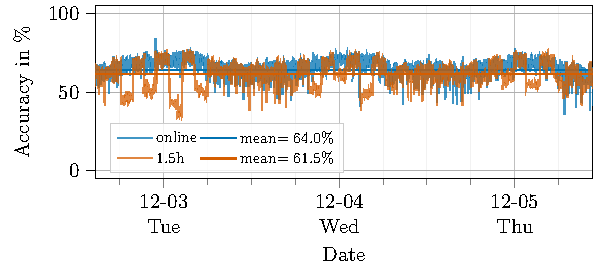
\includegraphics[width=0.85\linewidth, page=1]{pdf/c_6.pdf}%
        \label{fig_first_case}}
    \hfil
        \subfloat[The 3h window size performance comparison.]{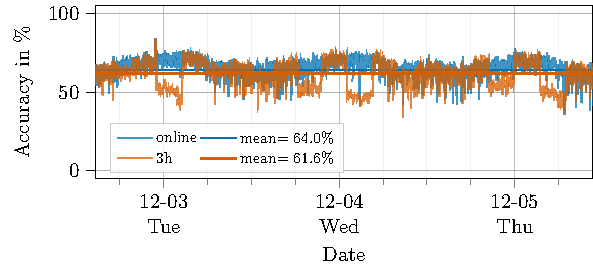
\includegraphics[width=0.85\linewidth, page=1]{pdf/c_12.pdf}%
        \label{fig_second_case}}
    \hfil
        \subfloat[The stacking ensemble performance comparison.]{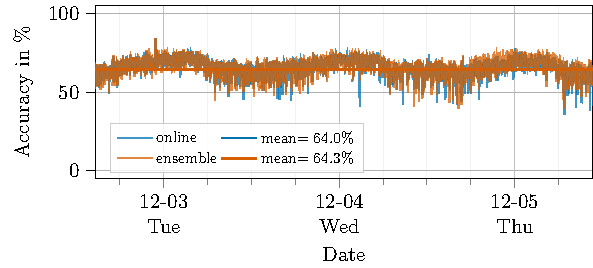
\includegraphics[width=0.85\linewidth, page=1]{pdf/online_ensemble_graph.pdf}%
        \label{fig_third_case}}
    \caption{The mean accuracy measured for each incoming block of flows and the overall mean accuracy for all flows within the selected time period.}
    \label{fig:online_offline_comparison}
\end{figure}

\section{Conclusion and Future Work}

At the beginning, a short overview of related work was given, in which on the one hand network flow prediction and on the other hand the utilization of a time-window concept for the improvement of machine learning algorithms was addressed. To the best of our knowledge, this work represents a novelty at the current time that combines the two topics thematically. For this purpose, an already existing architecture for flow prediction was extended such that, firstly, several windowed base learners can be operated in parallel and their results can be combined in a meta learner. Secondly, the classification is now performed in a true online manner, resulting in more application-oriented test outputs than in previous evaluations. For the presented architecture, the code was provided and the experimental framework parameters were described in detail to ensure the reproducibility of the results. Subsequently, the proposed approach was experimentally investigated by measuring performance differences in terms of prediction accuracy in the context of the bit rate of a flow. A subsequent analysis of the results showed that no significant improvements were achieved with the proposed approach in this particular configuration. Based on this, the following issues are considered for future work.

\begin{itemize}
    \item Performing a dataset analysis, which examines concept changes over time, should reveal points of improvement in the algorithm.
    \item More extensive experiments with greater variation in window sizes, should provide better insight into the approach.
    \item Introducing a temporal aspect into the feature space of the Level 1 classifier, by using the flow timestamps, and processing it via a Recurrent Neural Network could recognize temporal dependencies between windows.
    \item An algorithm for dynamically determining window sizes based on the performance of individual level 0 classifiers would provide flexibility in adapting to the data stream. 
    \item Besides the separation of the ensemble into different time scales, bagging the feature space in order to diversify the ensemble's base models could improve the general performance of the stacking ensemble.
    \item Focusing solely on improving the prediction of a flow's bit rate, which is the main challenge in this setup, a stacking ensemble based on level 0 classifiers, each operating on a different label, could be a promising concept. Thus, combining the results of the prediction of the number of packets, the number of bytes, and the duration of a flow could achieve an accurate bit rate prediction.
\end{itemize}

\newpage

\bibliographystyle{IEEEtran}
\bibliography{IEEEabrv,literature}

\end{document}


